\documentclass[10pt,twocolumn,letterpaper]{article}
\usepackage[T1]{fontenc}
\usepackage[utf8]{inputenc}
\usepackage[letterpaper,textwidth=6.875in,textheight=8.875in,columnsep=0.3125in,top=1in,headheight=0pt,headsep=0pt]{geometry}
\usepackage{times}
\usepackage{graphicx}
\usepackage{booktabs}
\usepackage{array}
\usepackage{tabularx}
\usepackage{ragged2e}
\usepackage{caption}
\usepackage{enumitem}
\usepackage{microtype}
\usepackage{pifont}
\usepackage{amssymb}
\usepackage[dvipsnames]{xcolor}
\usepackage{titlesec}
\usepackage[hidelinks]{hyperref}
\usepackage{morefloats}
\extrafloats{60}
\renewcommand{\arraystretch}{1.15}
\setlength{\parindent}{1em}\setlength{\parskip}{2pt}
\titleformat{\section}{\normalfont\large\bfseries}{}{0pt}{}
\titleformat{\subsection}{\normalfont\normalsize\bfseries}{}{0pt}{}
\titleformat{\subsubsection}{\normalfont\normalsize\itshape\bfseries}{}{0pt}{}
\titlespacing*{\section}{0pt}{10pt}{4pt}
\titlespacing*{\subsection}{0pt}{8pt}{3pt}
\titlespacing*{\subsubsection}{0pt}{6pt}{2pt}
\newenvironment{quotebox}%
 {\par\vspace{3pt}\noindent\begin{list}{}{\setlength{\leftmargin}{1em}\setlength{\rightmargin}{0.5em}}\item\footnotesize\itshape\color{black!80}\hspace*{-0.6em}\vrule width 2pt\hspace{0.6em}\ignorespaces}%
 {\end{list}\vspace{3pt}}
\captionsetup{font=footnotesize,labelformat=empty,skip=2pt}
\title{\vspace{-1.2em}\textbf{Reference-Driven Agentic Short-Form Video Generation System}\\[2pt]
\large Methodology and Evaluation --- Working Draft (Chapters 3--4, v0.1)}
\author{MSc AI for Media \quad\textbullet\quad NCCA, Bournemouth University\\
\texttt{Draft compiled 2026-07-17}}
\date{}
\begin{document}
\maketitle
{\centering\large\bfseries Chapter 3 --- Methodology and System Design\par}\vspace{4pt}

\begin{quotebox}\textbf{Draft status:} First draft (v0.1). Grounded in the locked four-stage architecture and the \texttt{live\_test\_03\_4shots} reference run (2026-07-17). Tense convention used throughout: the \textbf{present tense} describes the \emph{designed} system; where a mechanism is designed but not yet executed on the reported run, this is stated explicitly rather than implied as complete. See \S{}3.9 for a consolidated implementation-status table.\end{quotebox}

\section*{3.1 Motivation and design rationale}

\subsection*{3.1.1 From interactive assistance to reproducible orchestration}

A useful way to frame this system's contribution is by contrast with how the same creative task is carried out inside a hosted conversational image assistant (for example, ChatGPT's image mode). There, a user uploads a few images and issues a terse instruction --- \emph{"keep this person, put her in a street scene, in this outfit"} --- and a satisfactory result appears, often after a little back-and-forth. What is invisible to the user is that the assistant performs a series of steps \textbf{implicitly}, behind the conversational interface: it interprets each image (which region is the face, which is clothing, which is background), it carries the running intention ("stay this person") across turns, it expands the terse instruction into a stronger visual prompt, it decides which reference should dominate, and --- crucially --- it can \emph{see its own output} and revise on the next turn.

The OpenAI Images API exposes only the generation primitive that sits underneath such an experience. \texttt{images.edit} accepts one or more source images plus a prompt and returns an edited image; it does \textbf{not} know that one input is meant to fix composition, another only the face, or that identity must be preserved above outfit. Absent explicit instruction, multiple conditioning images \emph{compete for control} and the model settles on a compromise --- a recurring failure mode being that the scene and the outfit come through while the \textbf{face drifts}. The orchestration that a hosted assistant hides therefore has to be rebuilt, explicitly, outside the API.

This is precisely where the contribution lies, and it must be stated correctly. The goal is \textbf{not} to reproduce a hosted assistant's hidden helper. That helper is \emph{opaque} (its choices cannot be inspected), \emph{non-reproducible} (the same request may weight references differently on different runs), and \emph{non-measurable} (it returns no score for whether identity was preserved). This system instead turns each hidden step into an \textbf{explicit, reproducible, auditable and measurable} component of an agentic orchestration layer around the image API: the API generates, and the system decides, constrains, organises and repairs. The creative outcome is re-cast as an engineering pipeline whose every decision is logged (\S{}3.7) and whose output quality is scored (\S{}3.6) --- which is what makes it valid both as a dissertation artefact and as evidence of applied agentic engineering, rather than a one-off interactive result.

Table 3.1 maps each implicit step to the explicit component that realises it here.

\begin{table*}[t]
\centering
{\footnotesize\textbf{\textbf{Table 3.1 --- Implicit hosted-assistant steps vs. explicit pipeline components}}}\par\vspace{3pt}
\footnotesize
\begin{tabularx}{\textwidth}{>{\RaggedRight\arraybackslash}X>{\RaggedRight\arraybackslash}X}
\toprule
Implicit step (hosted assistant) & Explicit component (this system) \\
\midrule
Understand image content (face / outfit / background) & GPT-4o Vision semantic pass + source-frame structural anchor (Stage 1) \\
Hold the running "keep this person" intention & Identity anchor + locked \texttt{images.edit} slot order (slot \texttt{[0]} primary) \\
Expand a terse instruction into a strong visual prompt & Block-structured prompt (CHARACTER / LOOK / SCENE / FRAMING) \\
Decide which reference dominates & Fixed slot priority + input separation (identity / look / scene / source frame) \\
Suppress unwanted content & Forbidden-word guard (positive-only prompt; negatives stored, never sent) \\
"It doesn't look right --- try again" & Human review gate + decision log + evaluation$\rightarrow$repair loop \\
See the result and judge it & Evaluator: ArcFace identity, DWPose pose, framing, beat --- a \emph{score}, not a feeling \\
\bottomrule
\end{tabularx}
\end{table*}

The rest of this chapter details these components. The difference to keep in view is that where the hosted assistant \emph{feels} whether a result is right, this system \emph{measures} it (\S{}3.6) and records the decision (\S{}3.7), converting an opaque interaction into reproducible, evaluable evidence.

\subsection*{3.1.2 Design principles}

The system is built as a \textbf{four-stage agentic pipeline} organised around a single, human-readable state file rather than as a linear generator or an ensemble of chat agents. The design follows one governing principle:

\begin{quotebox}\textbf{Tools compute; agents decide.}\end{quotebox}

Deterministic tools (shot-cut detection, beat tracking, pose estimation, face embedding, rendering) produce measurable signals. Language-model agents (Template Builder, Generation Planner, Evaluator, Repair Decision-Maker) consume those signals and take structured decisions that are written back to the state file. This separation is what allows the pipeline's behaviour to be audited: every decision is a logged transition over shared state, not an opaque conversation.

The task is framed narrowly and deliberately. It is \textbf{reference-video decomposition + IP-conditioned regeneration + an automatic evaluation--repair loop} --- not a general "AI watches a video and makes a video" generator. The reference video is analysed only for \emph{formal structure} (shot cuts, rhythm, framing, body orientation, timing); no reference pixels or reference audio appear in the output. This scoping is both a technical decision (structure is measurable and reusable; content is not) and a copyright decision (\S{}3.8).

The single feature that makes the system \emph{agentic} rather than a fixed pipeline is the feedback edge from Stage 4 back to Stage 3: \textbf{Evaluation $\rightarrow$ Generation}. A shot that fails evaluation is diagnosed and only that shot is regenerated, guided by the diagnosis. The rest of the sequence is untouched. Without this edge the system would be a one-shot generator; with it, the system reasons about its own output and repairs selectively.

\section*{3.2 System architecture}

The pipeline has four stages and one shared artefact:

\begin{enumerate}[leftmargin=1.4em,itemsep=1pt,topsep=2pt]

\item \textbf{Reference Analysis} --- extract shot cuts, beats, camera-motion class, pose/motion, and framing from the reference video using deterministic tools.

\item \textbf{Template Builder} --- synchronise shot cuts, pose timestamps and audio beats into a single \textbf{beat-aligned storyboard JSON}.

\item \textbf{IP-Conditioned Generation} --- generate each shot from the fixed IP character plus a per-shot scene prompt, keyframe-first, then image-to-video, then assemble.

\item \textbf{Evaluation \& Repair} --- score each shot on identity, pose/motion, framing and beat alignment; on failure, diagnose and regenerate only the failing shot.

\end{enumerate}

All four stages read from and write to \textbf{\texttt{project\_state.json}}, the central state file (\S{}3.7). The system is delivered as a single Flask dashboard exposing two input modes that share this architecture: \textbf{Mode A} (reference video $\rightarrow$ shot analysis $\rightarrow$ IP-conditioned photoreal regeneration) and \textbf{Mode B} (natural-language prompt $\rightarrow$ animated storyboard sheet $\rightarrow$ panel review $\rightarrow$ JSON $\rightarrow$ video). This chapter documents Mode A, which exercises the full reference-decomposition pipeline; Mode B is described as a scoped variant in \S{}3.8.

\begin{figure*}[t]
\centering
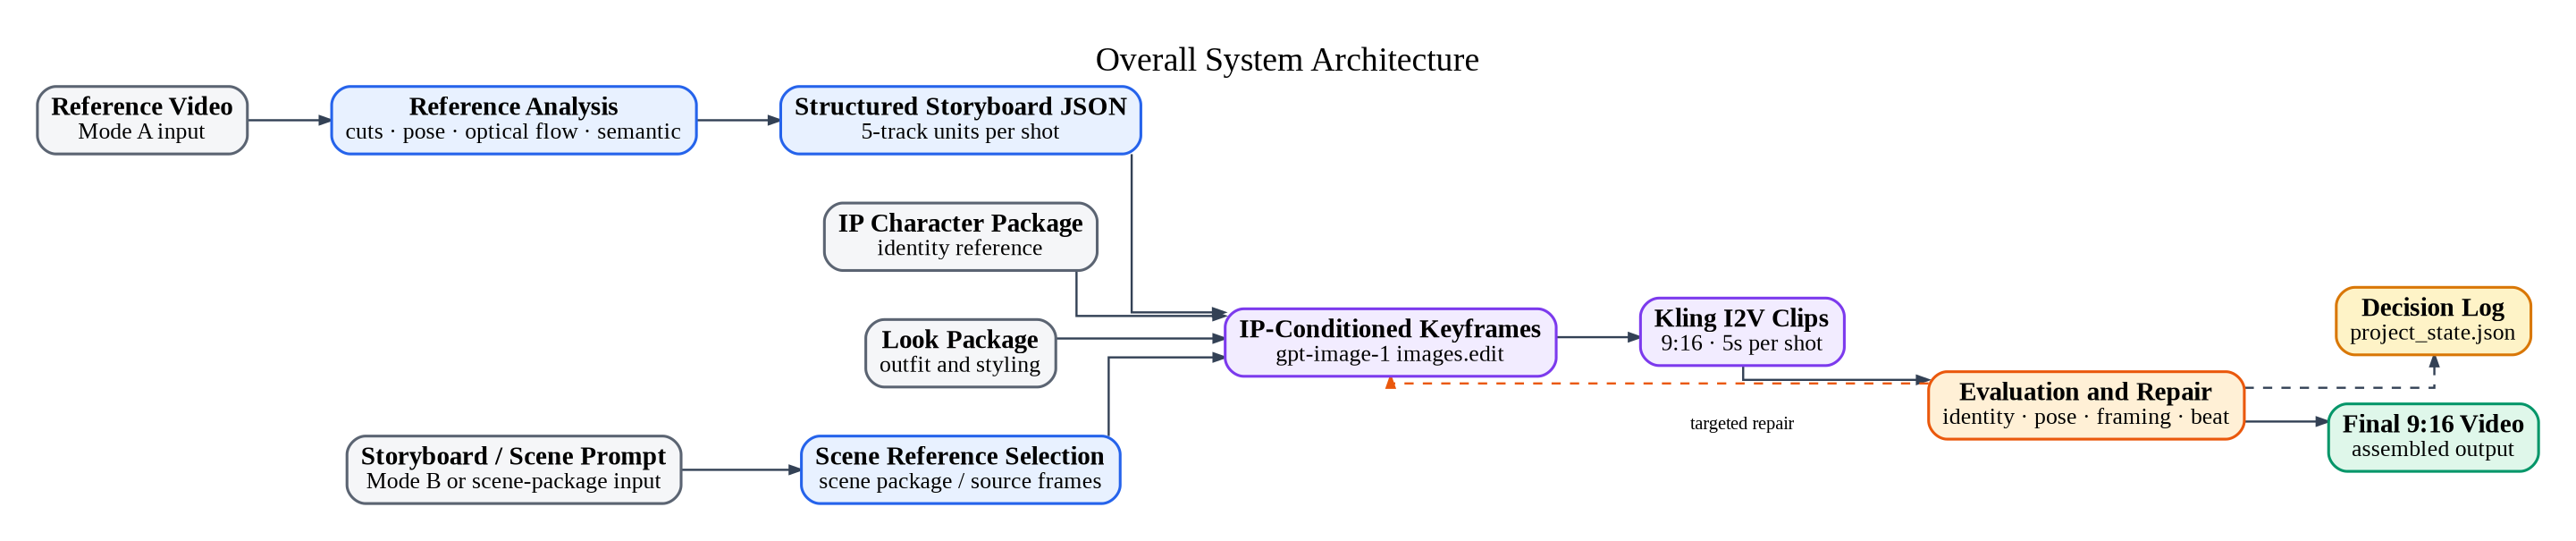
\includegraphics[width=\textwidth]{figs/overall_system_architecture_optimized.png}
\par\vspace{3pt}{\footnotesize \textbf{Figure 3.1} --- Overall system architecture: reference video $\rightarrow$ structured storyboard JSON $\rightarrow$}
\end{figure*}

IP-conditioned keyframes $\rightarrow$ Kling I2V clips $\rightarrow$ evaluation \& repair, with the targeted-repair edge back into keyframe generation and the decision log written to \texttt{project\_state.json}.

\section*{3.3 Stage 1 --- Reference Analysis}

Stage 1 converts the reference clip into structured, per-shot signal. It runs a bank of deterministic tools and merges their outputs conservatively; it does \textbf{not} ask a language model to guess shot boundaries or motion.

\begin{table*}[t]
\centering
\footnotesize
\begin{tabularx}{\textwidth}{>{\RaggedRight\arraybackslash}X>{\RaggedRight\arraybackslash}X>{\RaggedRight\arraybackslash}X}
\toprule
Signal & Tool / method & Output \\
\midrule
Shot cuts & PySceneDetect & Cut list with timestamps \\
Beats / tempo & librosa & Beat grid, BPM \\
Camera motion & Optical-flow classifier & Discrete camera-motion class (e.g. push-in, static) \\
Pose / character motion & MediaPipe keypoints & Per-shot body orientation and motion type \\
Semantic description & GPT-4o Vision & Framing / content labels per shot \\
\bottomrule
\end{tabularx}
\end{table*}

On the reference run, a 7.92 s, 30 fps, 123 bpm four-shot beach-sunset clip was decomposed into \textbf{four shots} with per-shot duration, framing class and camera-motion class. Signals from independent tools are combined by a \textbf{conservative multi-signal merge}: where tools disagree, the pipeline prefers the more reliable structural signal (the detected cut) over weaker inferred signals, rather than averaging them. This keeps the extracted template honest about what was actually measured.

Two properties of Stage 1 are load-bearing for the honesty of the whole system. First, camera motion and character motion are \textbf{estimated heuristically} --- the optical-flow class and the MediaPipe-derived motion type are categorical, not exact trajectories. Second, the semantic layer (GPT-4o Vision) is used only for description and enrichment; it never overrides a deterministic measurement. These are stated as limitations in the evaluation chapter, not hidden.

\begin{figure*}[t]
\centering
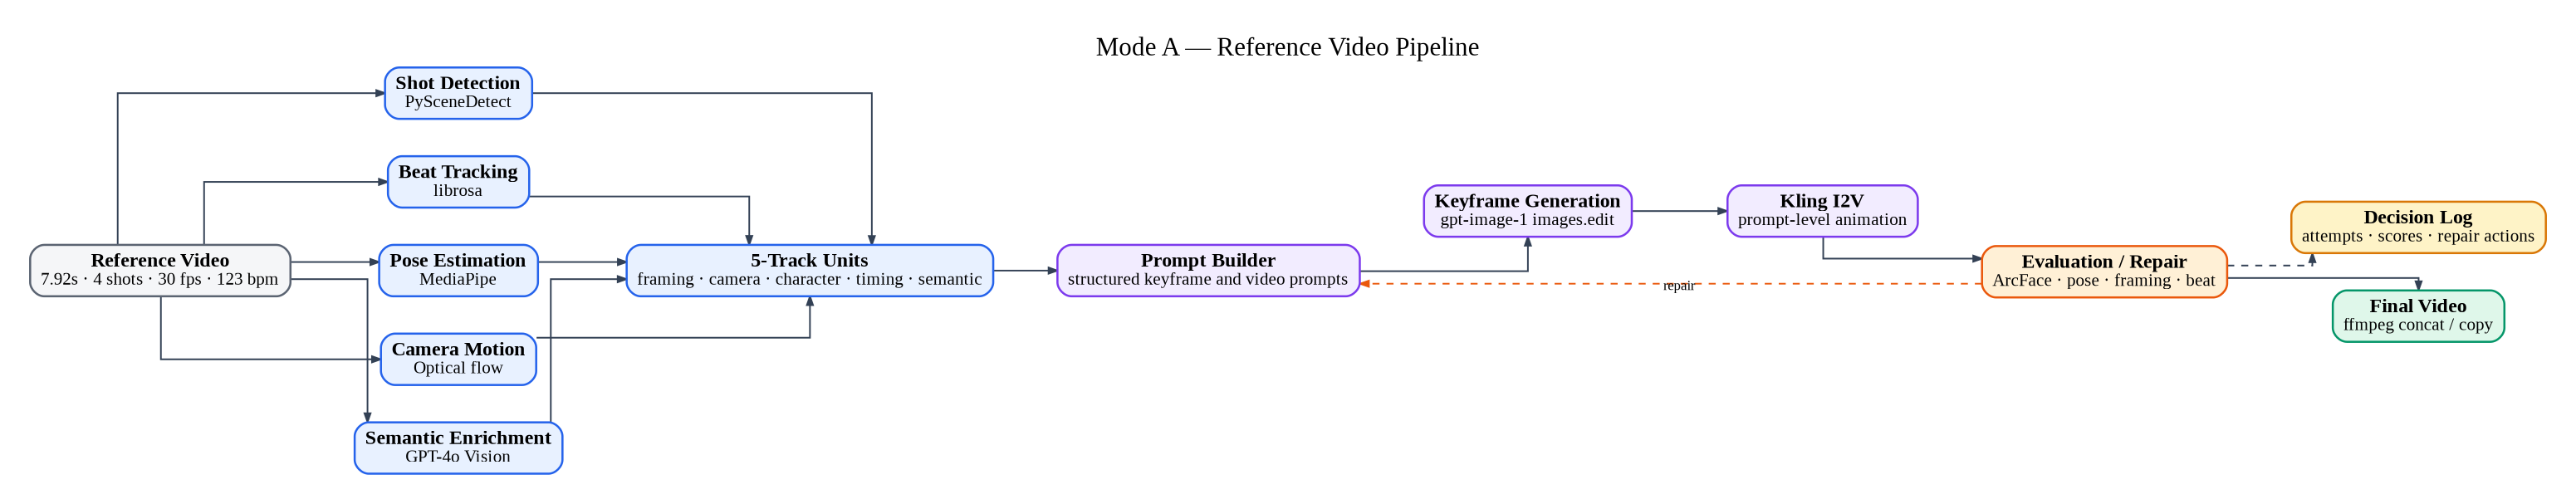
\includegraphics[width=\textwidth]{figs/mode_a_reference_video_pipeline_optimized.png}
\par\vspace{3pt}{\footnotesize \textbf{Figure 3.2} --- Mode A reference-video pipeline: the deterministic analysis bank}
\end{figure*}

(PySceneDetect, librosa, MediaPipe, optical flow, GPT-4o Vision) feeds the 5-track units and prompt builder, then keyframe generation, Kling I2V, evaluation/repair, and ffmpeg assembly.

\section*{3.4 Stage 2 --- Template Builder (beat-aligned storyboard)}

Stage 2 is the contribution that is easy to under-sell as "format conversion" but is not. It takes three time-stamped signal streams --- \textbf{shot cuts}, \textbf{pose timestamps} and \textbf{audio beats} --- and synchronises them into a single beat-aligned storyboard JSON. Each shot becomes a \textbf{generation unit} carrying five parallel tracks:

\begin{itemize}[leftmargin=1.2em,itemsep=1pt,topsep=2pt]

\item \texttt{framing} --- shot size / composition

\item \texttt{camera\_motion} --- camera-motion class from Stage 1

\item \texttt{character\_motion} --- body orientation / motion type

\item \texttt{timing} --- shot duration and its position on the beat grid

\item \texttt{semantic} --- content / scene description

\end{itemize}

On the reference run all four units reached \texttt{track\_completeness = full}.

The alignment step snaps shot cuts to the nearest audio beat, but under an explicit \textbf{maximum snap distance}. If a cut lies within the threshold of a beat, it is snapped and the timing is beat-locked; if the nearest beat is \emph{too far}, the \textbf{original cut is kept} rather than forcing a musically wrong alignment. This guard is deliberate: forcing every cut onto a beat would corrupt the timing of shots that were never beat-driven in the reference. The storyboard therefore records, per shot, whether its timing is beat-locked or cut-preserved --- this distinction later feeds the beat-alignment metric in Stage 4.

\begin{figure*}[t]
\centering
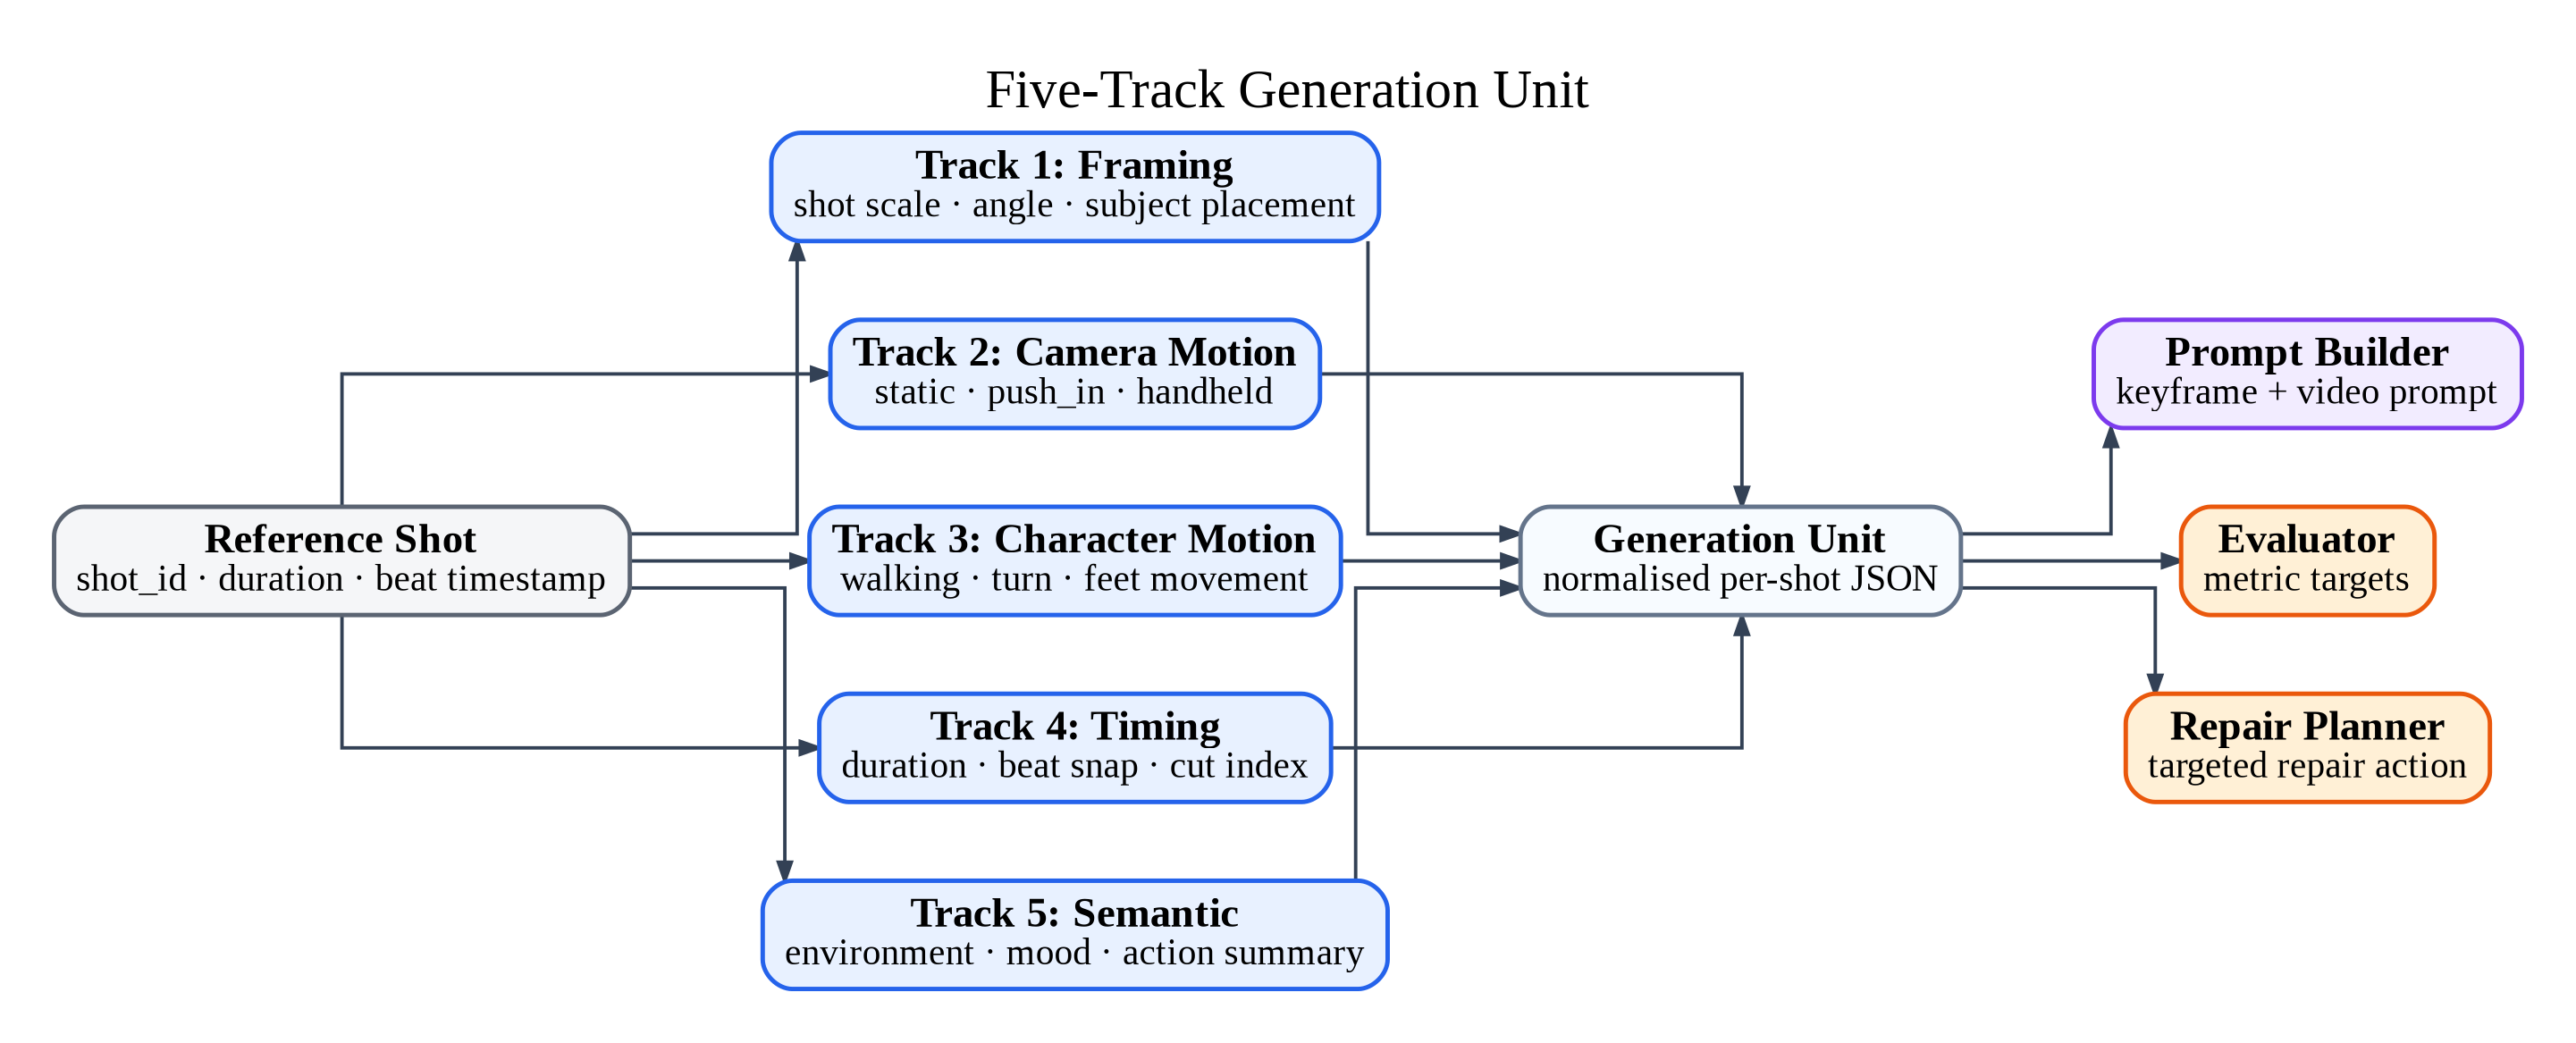
\includegraphics[width=\textwidth]{figs/five_track_generation_unit_optimized.png}
\par\vspace{3pt}{\footnotesize \textbf{Figure 3.3} --- Five-track generation unit: each reference shot (\texttt{shot\_id}, duration, beat}
\end{figure*}

timestamp) expands into framing, camera-motion, character-motion, timing and semantic tracks, normalised into a per-shot JSON that feeds the prompt builder, evaluator and repair planner.

\section*{3.5 Stage 3 --- IP-Conditioned Generation}

Stage 3 regenerates each shot with the fixed IP character in the new scene. It is \textbf{keyframe-first}: the pipeline first produces one approved keyframe per shot, then animates that keyframe to a clip, then assembles the clips. Generation is always \textbf{per-shot, never one-shot-whole-video}, so that a single failed shot can be repaired without re-rolling the sequence.

\subsection*{3.5.1 Identity / look / scene / source-frame separation}

A shot's conditioning is factored into four independent sources so that each can be controlled and, on failure, adjusted in isolation: the \textbf{IP identity} (who the character is), the \textbf{look} (the specific outfit/styling for this run), the \textbf{scene} (environment/lighting), and the \textbf{source frame} (structural anchor from the reference). Keeping these separate is what lets the repair layer target one axis --- e.g. fix the outfit without disturbing identity or framing.

\begin{figure*}[t]
\centering
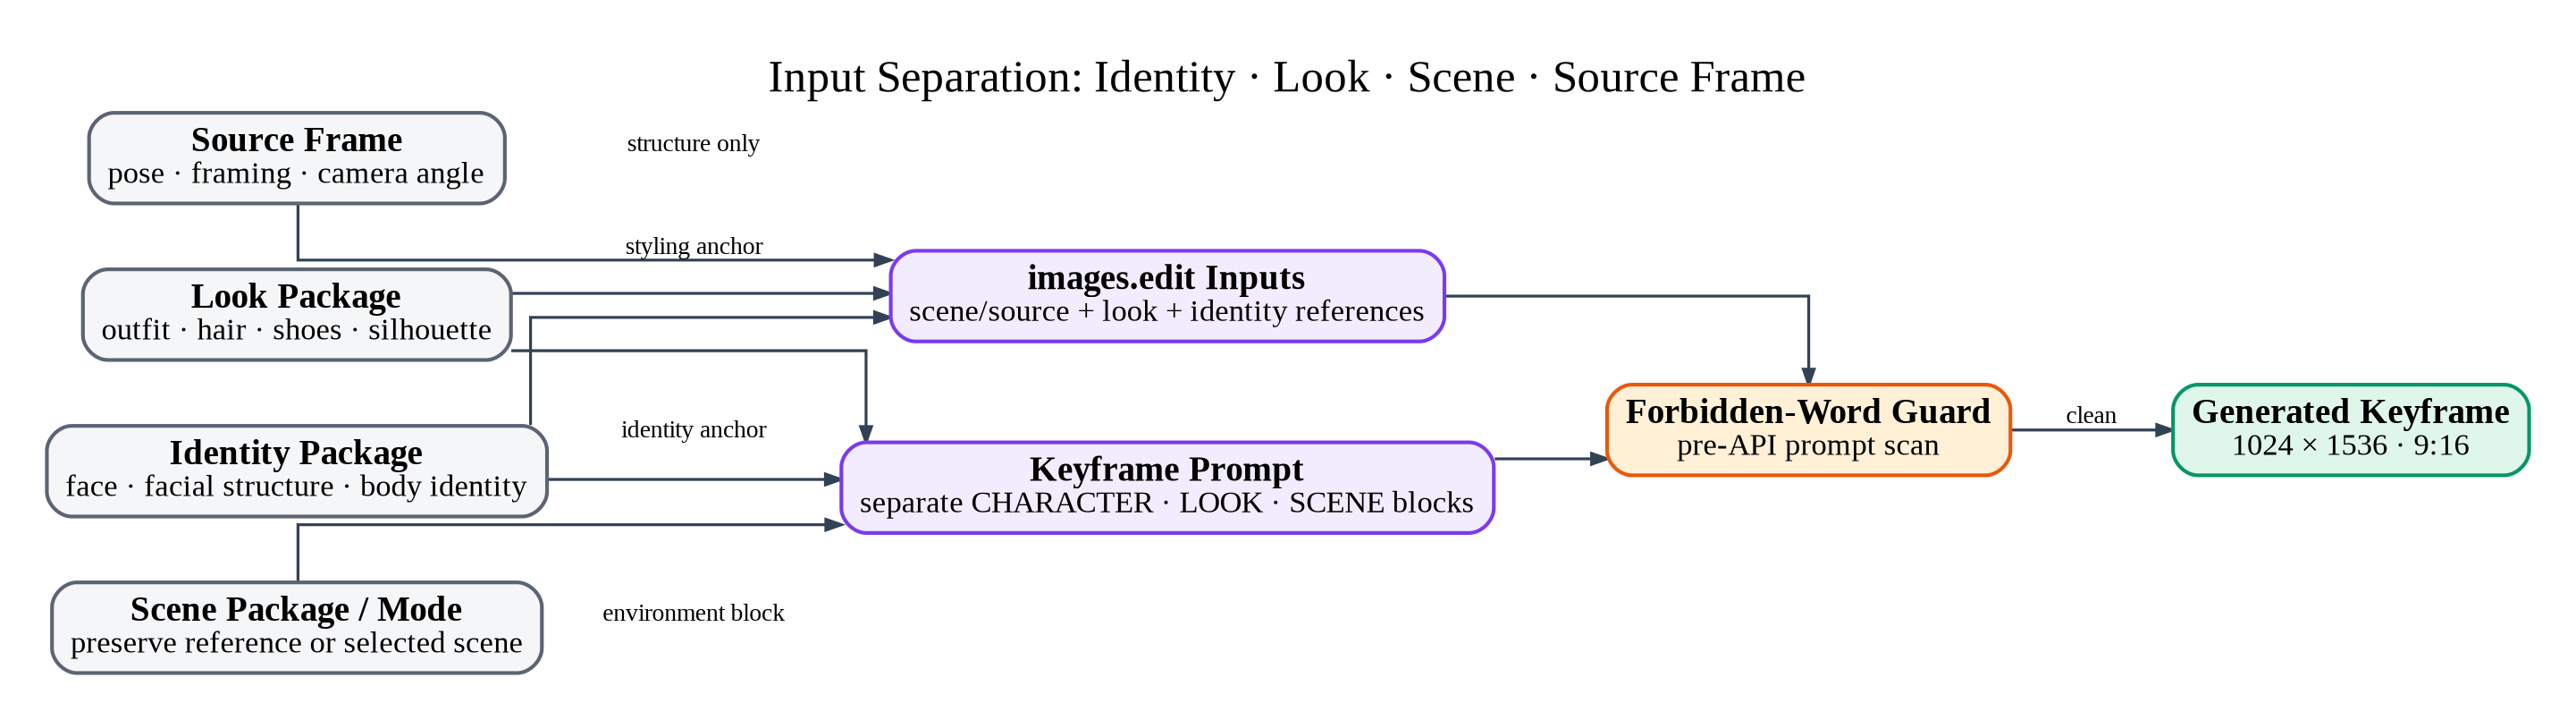
\includegraphics[width=\textwidth]{figs/identity_look_scene_source_frame_separation_optimized.png}
\par\vspace{3pt}{\footnotesize \textbf{Figure 3.4} --- Input separation: source frame (structure only), look package, identity}
\end{figure*}

package and scene package/mode are kept as independent conditioning sources feeding the \texttt{images.edit} inputs and the block-structured keyframe prompt, gated by the forbidden-word guard.

\subsection*{3.5.2 Keyframe generation}

Keyframes are generated with \texttt{gpt-image-1} via the \texttt{images.edit} endpoint at 1024$\times$1536, medium quality. Each keyframe is conditioned on \textbf{four input images in a locked slot order}:

\begin{table*}[t]
\centering
\footnotesize
\begin{tabularx}{\textwidth}{ll>{\RaggedRight\arraybackslash}X}
\toprule
Slot & Content & Role \\
\midrule
\texttt{[0]} & Source frame & \textbf{Primary} structural anchor (framing, body scale, camera distance) \\
\texttt{[1]} & Look front/body & Outfit reference \\
\texttt{[2]} & Look sheet & Look overview \\
\texttt{[3]} & Look close-up & Face reference \\
\bottomrule
\end{tabularx}
\end{table*}

The slot order is fixed because slot \texttt{[0]} carries the strongest structural weight; anchoring on the source frame is what preserves the reference's composition while the character and scene are replaced. One principled exception was applied on the reference run: for a \textbf{feet-only shot} (shot\_003) where the face is out of frame, the face close-up was left in the weakest slot \texttt{[3]} to avoid "face-bleed" into a shot that should contain no face.

Scene continuity is controlled by a \texttt{scene\_mode} flag. The reference run used \texttt{scene\_mode = preserve\_reference\_scene}, so the beach-sunset environment, wet sand, warm amber light and ocean horizon were rendered consistently across all four keyframes with no stale scene prompts injected.

A \textbf{forbidden-word guard} runs on every keyframe prompt. Only a positive prompt is sent to the image API; the negative prompt (identity-drift and unwanted-content terms) is stored separately in state and \textbf{never} passed to the API. This both satisfies the image model's input contract and keeps a clean, auditable record of what was and was not requested. On the reference run this guard is itself part of the decision log: shot\_002's first attempt was blocked pre-API because bridal terms sat in the negative instructions, and was resolved by separating positive from negative language.

\begin{figure*}[t]
\centering
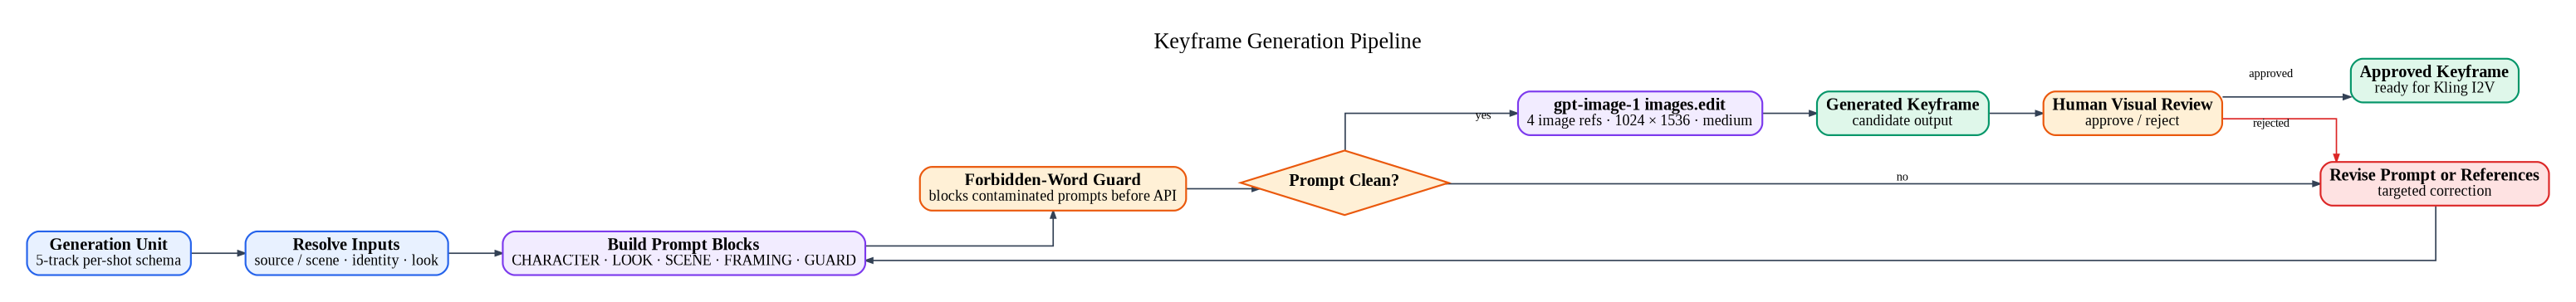
\includegraphics[width=\textwidth]{figs/keyframe_generation_pipeline_optimized.png}
\par\vspace{3pt}{\footnotesize \textbf{Figure 3.5} --- Keyframe generation pipeline, including the forbidden-word guard (blocks}
\end{figure*}

contaminated prompts before the API) and the human visual review approve/reject gate that routes rejected candidates to a targeted prompt/reference revision --- the keyframe-approval loop that operated on the reference run (\S{}3.7).

\subsection*{3.5.3 Image-to-video and assembly}

Each approved keyframe is animated with \textbf{Kling v1.6} (standard mode, 9:16, 5 s clips) driven by a natural-language \textbf{video prompt} describing the intended motion (walk direction, camera movement, body pose). Clips are concatenated by \texttt{ffmpeg} with stream copy (no re-encode) into the final vertical short (768$\times$1152 / 20.4 s on the reference run).

An honesty boundary is fixed here and carried into every claim about the system:

\begin{quotebox}\textbf{The system preserves reference shot structure and action intent, but does not perform exact frame-level motion transfer.}\end{quotebox}

Motion is \textbf{prompt-level image-to-video}, not skeleton- or optical-flow-conditioned pose transfer. No per-frame keypoint sequence, ControlNet pose map or flow field is transmitted to the video model. Step cadence, exact stride length and inter-frame body position are therefore not controlled; only action \emph{intent} is. This is the designed behaviour of the current Mode A pipeline, and it reflects a deliberate scoping decision discussed next.

\begin{figure*}[t]
\centering
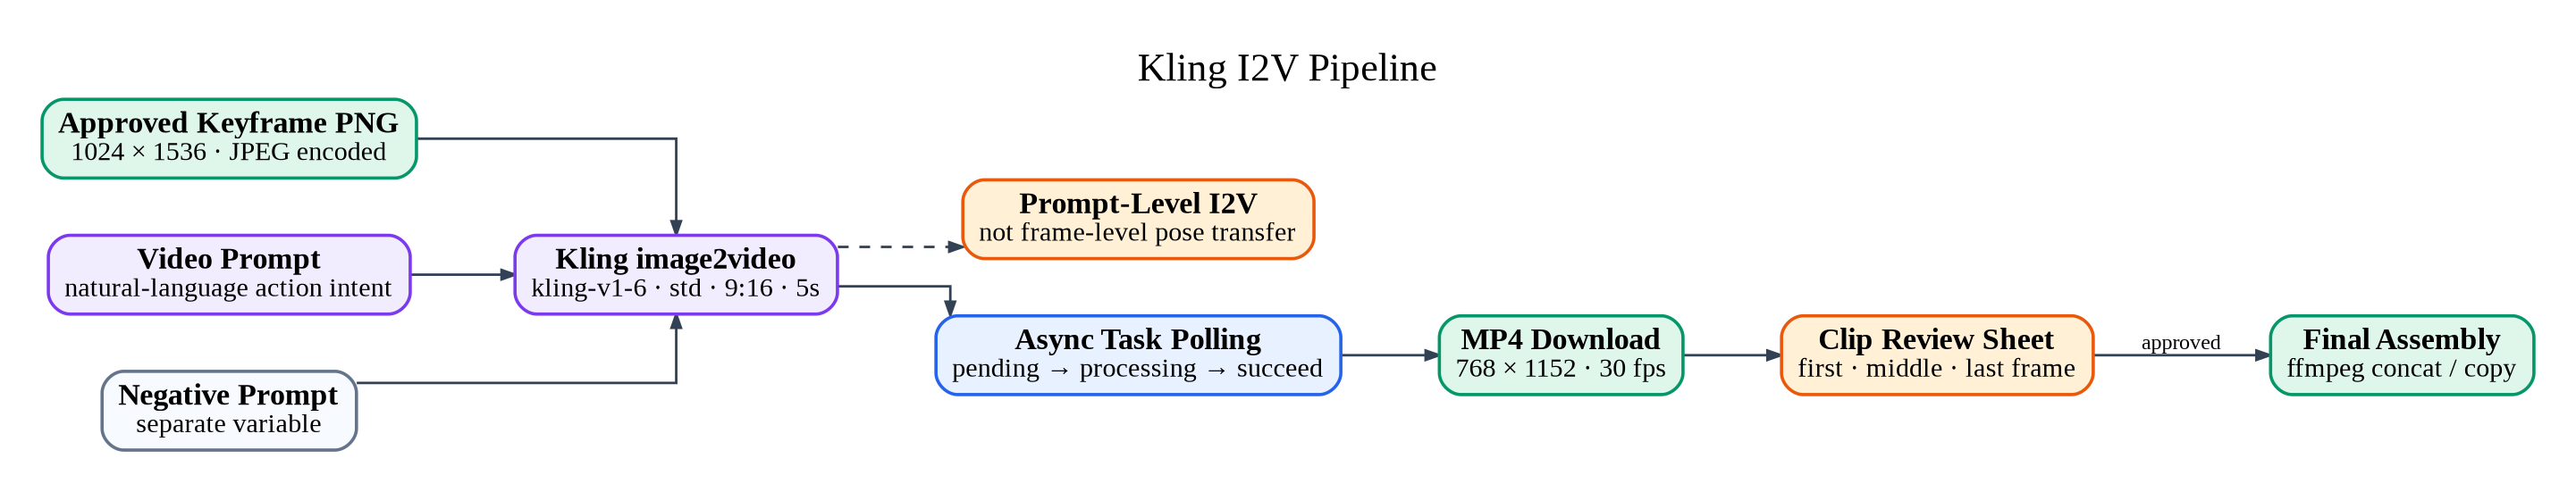
\includegraphics[width=\textwidth]{figs/kling_i2v_pipeline_optimized.png}
\par\vspace{3pt}{\footnotesize \textbf{Figure 3.6} --- Kling I2V pipeline: the approved keyframe (1024$\times$1536) plus a natural-language}
\end{figure*}

video prompt and a separately stored negative prompt drive \texttt{kling-v1-6} (prompt-level I2V, \emph{not} frame-level pose transfer); async polling $\rightarrow$ MP4 (768$\times$1152, 30 fps) $\rightarrow$ clip review $\rightarrow$ ffmpeg assembly.

\subsection*{3.5.4 Scoping note: pose control vs. identity}

The project's identified make-or-break risk is the tension between \textbf{strong pose conditioning} (which preserves motion) and \textbf{character identity} (which strong pose conditioning can distort). The planned Phase 0 feasibility test --- IP reference + pose skeleton + simple scene, checking that identity holds across poses against a pre-defined quantitative threshold --- was \textbf{not run} before the reference build. In line with the pre-committed fallback, the pipeline was therefore scoped to \textbf{keyframe-first generation with prompt-level I2V} rather than full skeleton-driven motion transfer. This is treated as a scoping decision, not a failure: a short-form vertical clip is, structurally, a sequence of key poses plus beat-driven cuts, and the keyframe-first route delivers that while sidestepping the identity-distortion risk of aggressive pose conditioning. Full pose-transfer is documented as future work (\S{}3.9), and the identity-vs-pose evaluation it would require is specified in \S{}3.6.

\section*{3.6 Stage 4 --- Evaluation and Repair}

Stage 4 is what closes the loop. It scores each generated shot, decides a verdict, and --- on failure --- diagnoses the cause and triggers a targeted regeneration of only that shot. The metrics are defined as follows:

\begin{table*}[t]
\centering
\footnotesize
\begin{tabularx}{\textwidth}{>{\RaggedRight\arraybackslash}X>{\RaggedRight\arraybackslash}X>{\RaggedRight\arraybackslash}X}
\toprule
Metric & Method & Interpretation \\
\midrule
IP identity consistency & Face-embedding (ArcFace) cosine distance, generated vs. IP reference & Lower distance = identity held \\
Pose / motion similarity & Keypoint distance (DWPose on generated keyframe) vs. source-frame pose & Lower = closer to reference motion \\
Framing accuracy & Composition / shot-size match vs. reference framing class & Match / mismatch \\
Beat alignment error & Cut timestamp vs. nearest beat, in ms & Smaller = tighter to the beat grid \\
\bottomrule
\end{tabularx}
\end{table*}

Two further run-level metrics are recorded: \textbf{regeneration success rate} (fraction of failing shots repaired within the retry budget) and \textbf{number of manual interventions} (\texttt{needs\_human} escalations).

\subsection*{3.6.1 Two-layer repair}

Repair is deliberately split into a base layer that must work and an enhanced layer that is a bonus:

\begin{itemize}[leftmargin=1.2em,itemsep=1pt,topsep=2pt]

\item \textbf{Base layer (guaranteed).} On failure: change seed / apply a small prompt tweak / regenerate, up to a maximum of \emph{N} retries. This guarantees the loop runs and produces ablation data even when diagnosis is unavailable.

\item \textbf{Enhanced layer (bonus).} On failure, classify the failure reason and apply a \emph{targeted} repair: identity drift $\rightarrow$ raise IP/LoRA conditioning weight; pose mismatch $\rightarrow$ strengthen pose conditioning; bad framing $\rightarrow$ rewrite the framing prompt; beat error $\rightarrow$ adjust cut timing. Diagnosis is treated as \emph{imperfect} and is itself evaluated (where it helps vs. where it misjudges); the dissertation does not depend on diagnosis being perfect, only on it being honestly assessed.

\end{itemize}

When retries hit the maximum and a shot still fails, it is moved to an explicit terminal state \textbf{\texttt{needs\_human}} --- the pipeline never leaves a shot resting on a bare "fail", and never loops indefinitely. \texttt{needs\_human} shots are counted as manual interventions in the evaluation.

\subsection*{3.6.2 Core experiment}

The central experiment is an \textbf{ablation of the loop itself}: run the pipeline with the evaluation--repair loop \textbf{OFF} (one-shot generation) versus \textbf{ON} (auto-detect failures + repair), and compare on the metrics above plus regeneration success rate and manual-intervention count. The loop-OFF condition is the baseline; the loop-ON condition tests whether selective, diagnosis-guided repair improves per-shot quality at acceptable cost.

\begin{figure*}[t]
\centering
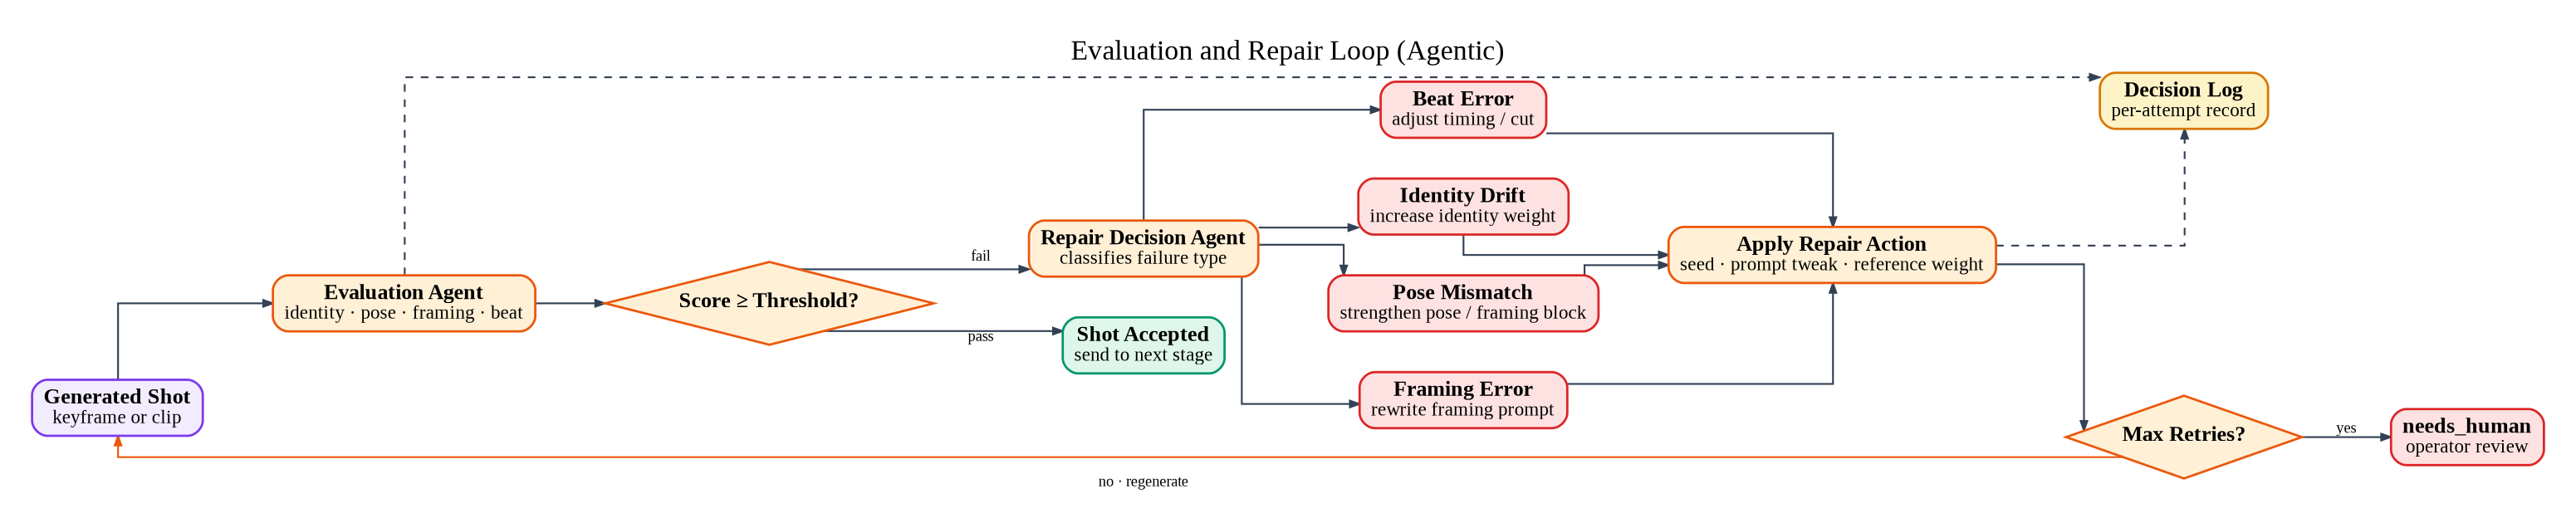
\includegraphics[width=\textwidth]{figs/evaluation_repair_loop_optimized.png}
\par\vspace{3pt}{\footnotesize \textbf{Figure 3.7} --- Evaluation and repair loop (agentic): the Evaluation Agent scores each shot;}
\end{figure*}

on pass the shot is accepted, on fail the Repair Decision Agent classifies the failure (identity drift / pose mismatch / framing error / beat error) and applies a targeted repair, logging every attempt; on reaching max retries the shot escalates to \texttt{needs\_human}.

\begin{figure*}[t]
\centering
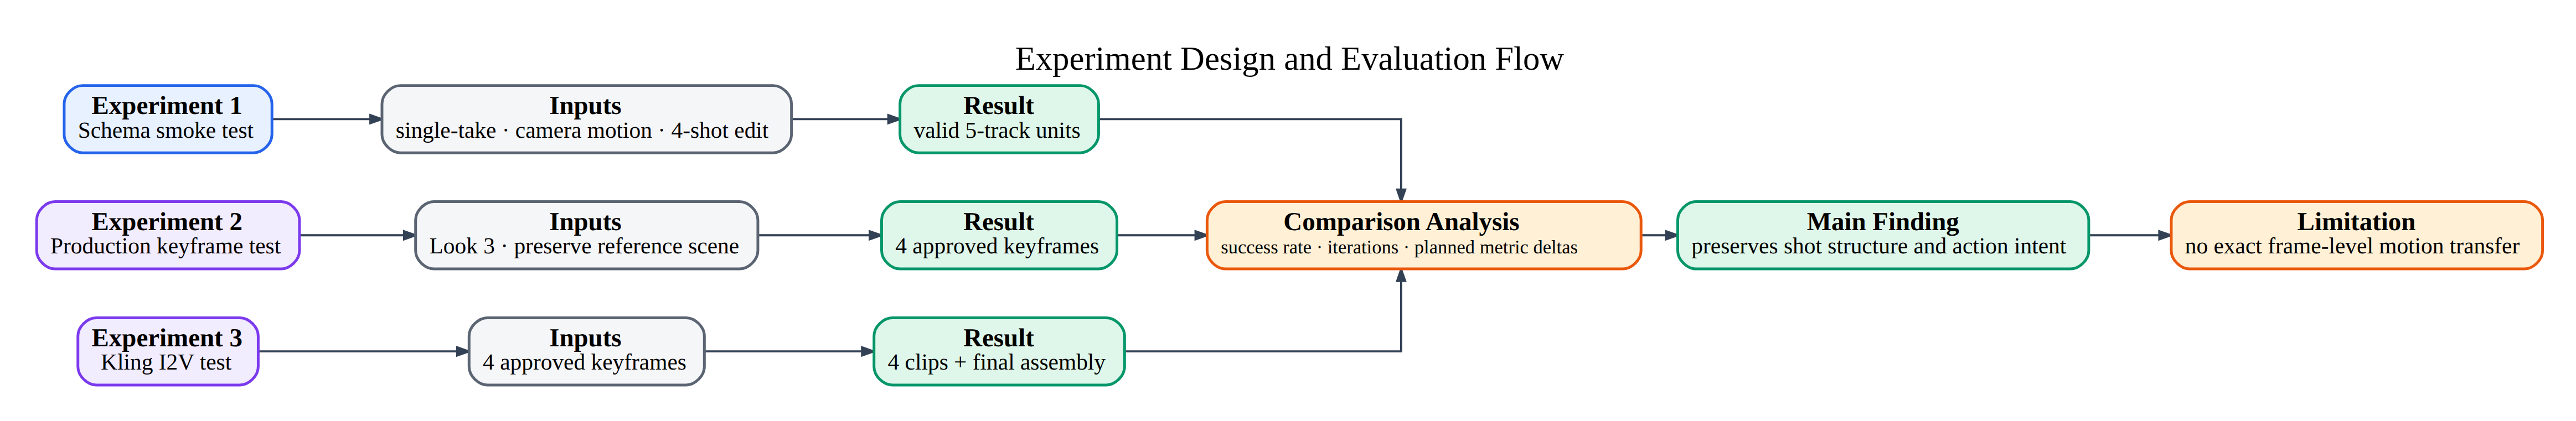
\includegraphics[width=\textwidth]{figs/experiment_evaluation_flow_optimized.png}
\par\vspace{3pt}{\footnotesize \textbf{Figure 3.8} --- Experiment design and evaluation flow: schema smoke test, production keyframe}
\end{figure*}

test and Kling I2V test feed a comparison analysis (success rate, iterations, metric deltas); main finding --- reference shot structure and action intent are preserved; limitation --- no exact frame-level motion transfer.

\subsection*{3.6.3 Loop trigger on the reported run (honest note)}

On \texttt{live\_test\_03\_4shots}, the automated scoring in this section was \textbf{not yet executed}: identity (ArcFace) and pose-keypoint (DWPose) distances were not computed on this batch, framing was assessed by human visual review, and the automatic repair loop was \textbf{not triggered}. The loop that \emph{did} operate on this run was the \textbf{keyframe-approval loop} --- a human-in-the-loop gate that diagnoses a failed keyframe and regenerates it before the shot is animated (\S{}3.7). The automated Stage-4 loop described above is the designed mechanism; \S{}3.9 states precisely what has and has not been run so that no evaluation claim outruns its evidence.

\section*{3.7 Central state file and decision log}

The pipeline's core is not "several agents chatting" but a single readable/writable \textbf{\texttt{project\_state.json}} that every stage transitions. Its most important element for this dissertation is the \textbf{per-shot decision log}, which is the concrete evidence that the system is agentic: each shot records its attempts, and each attempt records the action taken, the outcome, and --- where applicable --- the diagnosis that motivated the next attempt.

The reference run's decision log (\texttt{decision\_log.json}, schema \texttt{decision\_log\_v1}) demonstrates this at the keyframe stage. Each shot stores the model and slot configuration, the exact prompt used, the number of attempts, the issue encountered, and the fix applied:

\begin{table*}[t]
\centering
\footnotesize
\begin{tabularx}{\textwidth}{l>{\RaggedRight\arraybackslash}X>{\RaggedRight\arraybackslash}X>{\RaggedRight\arraybackslash}X>{\RaggedRight\arraybackslash}X}
\toprule
Shot & Keyframe attempts & Issue diagnosed & Repair action & Improved? \\
\midrule
shot\_001 & 1 & --- & v3 prompt (preserve scene, over-shoulder MCU) & approved first attempt \\
shot\_002 & 2 & v1 blocked by forbidden-word guard (bridal terms in negatives) & separate positive/negative prompts; v2 natural-realism language & yes \\
shot\_003 & 2 & v1 described a face-forward pose --- wrong for the source frame & inspect source frame $\rightarrow$ v2 rewritten as extreme low-angle feet close-up & yes \\
shot\_004 & 3 & v1--v2 rendered a generic business blazer, not the specified look & v3: labelled BLAZER/TIE/TROUSERS subsections + stronger negatives + look-front to slot \texttt{[1]} & yes \\
\bottomrule
\end{tabularx}
\end{table*}

This table is a \textbf{diagnose $\rightarrow$ act $\rightarrow$ re-evaluate} trace: each retry is a decision conditioned on an observed failure, not a blind re-roll. It is exactly the shape the automated Stage-4 loop is designed to produce, executed here through the human-approval gate. The decision log therefore doubles as dissertation evaluation data, and the same schema (attempts, scores, verdict, diagnosis, repair action, terminal \texttt{needs\_human}) is the container the automated loop writes into when it runs.

\section*{3.8 Copyright-aware workflow and Mode B}

\textbf{Copyright.} The workflow is designed so that no protected reference content can reach the output. References are authorised, self-created or royalty-free, and are analysed only for formal structure (rhythm, shot structure, generic motion, framing). Reference \textbf{audio} is used for beat analysis only and never appears in the output. Outputs use the original IP character, new scene prompts, and royalty-free or original assets. The governing intent is \textbf{"extract structure, regenerate content,"} never a re-skinned copy of the reference --- the reference run explicitly records that no reference pixels or audio are reproduced.

\textbf{Mode B (scoped variant).} Alongside the reference-video path, the same dashboard exposes a natural-language path: story prompt + template $\rightarrow$ GPT-4o panel plan $\rightarrow$ \texttt{gpt-image-1} animated storyboard sheet $\rightarrow$ panel review $\rightarrow$ storyboard JSON $\rightarrow$ core loop. Mode B is deliberately scoped --- \textbf{animation only, single character, no photoreal, no multi-strategy analysis} --- so that it demonstrates the storyboard-JSON-to-video half of the architecture without duplicating Mode A's reference-decomposition machinery.

\section*{3.9 Implementation status (what is built vs. what is designed)}

To keep every downstream claim bounded, the state of each stage on the reference run is stated explicitly:

\begin{table*}[t]
\centering
\footnotesize
\begin{tabularx}{\textwidth}{>{\RaggedRight\arraybackslash}Xl>{\RaggedRight\arraybackslash}X}
\toprule
Component & Designed & Executed on \texttt{live\_test\_03\_4shots} \\
\midrule
Reference analysis (cuts/beats/motion/pose/semantic) & \ding{51} & \ding{51} --- 4 shots from 7.92 s / 123 bpm \\
Beat-aligned storyboard, 5-track units & \ding{51} & \ding{51} --- all units \texttt{track\_completeness = full} \\
Keyframe-first IP-conditioned generation & \ding{51} & \ding{51} --- 4 keyframes approved \\
Kling prompt-level I2V + ffmpeg assembly & \ding{51} & \ding{51} --- 20.4 s, 768$\times$1152 final video \\
Keyframe-approval loop (human-in-the-loop, logged) & \ding{51} & \ding{51} --- decision log, 1/2/2/3 attempts \\
Automated Stage-4 scoring (ArcFace / DWPose / framing / beat) & \ding{51} & \ding{55} --- pending; not computed on this batch \\
Automated evaluation$\rightarrow$repair loop & \ding{51} & \ding{55} --- not triggered on this run \\
Phase 0 pose-vs-identity feasibility test & \ding{51} (planned) & \ding{55} --- not run; pipeline scoped to keyframe-first I2V \\
Loop ON vs OFF ablation (core experiment) & \ding{51} & \ding{55} --- pending automated scoring \\
\bottomrule
\end{tabularx}
\end{table*}

The foundation is valid on its own terms: a working reference-decomposition $\rightarrow$ beat-aligned storyboard $\rightarrow$ keyframe-first IP-conditioned generation $\rightarrow$ logged diagnose-and-retry loop, end to end, on a real four-shot run. The automated Stage-4 loop and its ablation are the immediate next work, and are the components whose \emph{design} --- not yet whose \emph{results} --- this chapter documents.

\emph{Draft v0.1 --- figures referenced by export name in \texttt{final/paper\_exports/diagrams/}. Chapter 4 (Evaluation \& Results) will report only metrics actually computed; anything marked \ding{55} above must not be reported as a result there.}

\clearpage
{\centering\large\bfseries Chapter 4 --- Evaluation and Results\par}\vspace{4pt}

\begin{quotebox}\textbf{Draft status:} First draft (v0.1). Reports the \texttt{live\_test\_03\_4shots} reference run (2026-07-17). \textbf{Reporting rule for this chapter:} only quantities that were actually measured are reported as results. Automated metric scores (identity, pose, framing, beat) were \textbf{not computed on this run} and are therefore presented as \emph{placeholders}, never as numbers. Every table below is explicitly labelled \textbf{Executed} or \textbf{Planned}. Video dimensions are stated as confirmed by \texttt{ffprobe}: \textbf{768$\times$1152, 30 fps, 20.4 s} (a vertical 2:3 short).\end{quotebox}

\section*{4.1 Aims and the meaning of "result" in this chapter}

The evaluation has two jobs. First, to establish that the pipeline runs \textbf{end to end} on a real reference and produces a coherent vertical short --- the \emph{system-works} result. Second, to specify the \textbf{automated, quantitative} evaluation that measures per-shot quality (identity, pose, framing, beat) and that drives the agentic repair loop --- the \emph{system-is-good} result.

At the time of writing, the first job is \textbf{done and verified}; the second is \textbf{designed, implemented in schema, and pending execution}. This chapter is deliberate about the boundary between the two. Where a result was produced by running the pipeline, it is reported as a result. Where a measurement is designed but has not been run, it is reported as a placeholder with an explicit \texttt{pending} status. No identity, pose, framing or beat score is invented, estimated, or implied.

A single claim boundary governs every result below and should accompany any demonstration of the system:

\begin{quotebox}\textbf{The system preserves reference shot structure and action intent, but does not perform exact frame-level motion transfer.}\end{quotebox}

\section*{4.2 Evaluation status at a glance}

Table 4.1 summarises what was executed versus what remains planned on the reference run. The detailed per-experiment results follow in \S{}4.3--\S{}4.6; the planned automated evaluation is specified in \S{}4.8--\S{}4.10.

\begin{table*}[t]
\centering
{\footnotesize\textbf{\textbf{Table 4.1 --- Executed vs. planned evaluation on \texttt{live\_test\_03\_4shots}}}}\par\vspace{3pt}
\footnotesize
\begin{tabularx}{\textwidth}{>{\RaggedRight\arraybackslash}Xl>{\RaggedRight\arraybackslash}X}
\toprule
Evaluation component & Type & Status on this run \\
\midrule
Schema smoke test (5-track unit completeness) & Executed & \ding{51} Complete \\
Keyframe generation (per-shot, human-approved) & Executed & \ding{51} 4/4 approved \\
Kling I2V clip generation & Executed & \ding{51} 4/4 succeeded \\
End-to-end assembly (final video) & Executed & \ding{51} 768$\times$1152, 20.4 s \\
Human visual review (identity/framing/look) & Executed & \ding{51} All shots approved \\
ArcFace identity scoring & Planned & \ding{55} Pending --- not computed \\
Pose-keypoint (DWPose) similarity & Planned & \ding{55} Pending --- not computed \\
Framing-accuracy metric & Planned & \ding{55} Pending --- visual only \\
Beat-alignment error (ms) & Planned & \ding{55} Pending --- not computed \\
Baseline (loop OFF) vs. agentic (loop ON) ablation & Planned & \ding{55} Pending --- automated loop not run \\
\bottomrule
\end{tabularx}
\end{table*}

The verified contribution of this run is therefore an \textbf{end-to-end generation success under human visual review}; the automated metric layer and its ablation are the next evaluation step (\S{}4.7, \S{}4.11).

\section*{4.3 Experiment 1 --- Schema smoke test}

\textbf{Type: Executed.} The schema smoke test checks that the reference-analysis and template-builder stages produce a structurally valid, per-shot storyboard --- i.e. that every detected shot expands into a complete five-track generation unit. This is the precondition for any downstream generation: an incomplete unit cannot be prompted or scored.

The reference clip (\texttt{test/test\_03\_multishot\_edit\_4shots.mp4} --- 7.92 s, 30 fps, 123 bpm) was decomposed into four shots, and all four produced full five-track units.

\begin{table*}[t]
\centering
{\footnotesize\textbf{\textbf{Table 4.2 --- Schema smoke test: 5-track unit completeness (Executed)}}}\par\vspace{3pt}
\footnotesize
\begin{tabularx}{\textwidth}{ll>{\RaggedRight\arraybackslash}X>{\RaggedRight\arraybackslash}X>{\RaggedRight\arraybackslash}X}
\toprule
shot\_id & Duration (s) & Framing class & Camera-motion class & Track completeness \\
\midrule
shot\_001 & 2.40 & Over-shoulder MCU (medium) & push\_in & full (5/5) \\
shot\_002 & 2.27 & Wide back-view (wide) & static & full (5/5) \\
shot\_003 & 2.13 & Extreme low-angle feet CU & handheld & full (5/5) \\
shot\_004 & 1.10 & Wide side-profile (wide) & handheld & full (5/5) \\
\bottomrule
\end{tabularx}
\end{table*}

\emph{Result:} 4/4 shots reached \texttt{track\_completeness = full}. The schema pipeline is validated; the storyboard JSON is well-formed and ready for generation. No generation-quality claim is made here --- this test concerns structural validity only.

\section*{4.4 Experiment 2 --- Keyframe generation attempts}

\textbf{Type: Executed.} Each shot's keyframe was generated with \texttt{gpt-image-1} (\texttt{images.edit}, 1024$\times$1536, medium) conditioned on four reference images in the locked slot order (source frame, look front, look sheet, look close-up). Every candidate passed through a pre-API forbidden-word guard and a human visual review gate; rejected candidates were diagnosed and regenerated with a targeted prompt/reference revision. Table 4.3 reports the per-shot attempt history exactly as recorded in \texttt{decision\_log.json} (schema \texttt{decision\_log\_v1}).

\begin{table*}[t]
\centering
{\footnotesize\textbf{\textbf{Table 4.3 --- Keyframe generation attempts and diagnose-and-repair actions (Executed)}}}\par\vspace{3pt}
\footnotesize
\begin{tabularx}{\textwidth}{ll>{\RaggedRight\arraybackslash}X>{\RaggedRight\arraybackslash}Xl}
\toprule
shot\_id & Attempts & Diagnosed issue & Repair action taken & Final status \\
\midrule
shot\_001 & 1 & --- & v3 prompt (preserve scene, over-shoulder MCU) accepted first pass & Approved \\
shot\_002 & 2 & v1 blocked pre-API by forbidden-word guard (bridal terms in negatives) & Separated positive/negative prompt; v2 natural-realism language & Approved \\
shot\_003 & 2 & v1 prompt described a face-forward pose --- wrong for the source frame & Inspected source frame; v2 rewritten as extreme low-angle feet close-up & Approved \\
shot\_004 & 3 & v1--v2 rendered a generic business blazer, not the specified look & v3: labelled BLAZER/TIE/TROUSERS subsections, stronger negatives, look-front $\rightarrow$ slot [1] & Approved \\
\bottomrule
\end{tabularx}
\end{table*}

\emph{Result:} 4/4 keyframes approved; total 8 generation attempts across 4 shots (mean 2.0 attempts/shot). Each retry was a decision conditioned on an observed, named failure --- a \textbf{diagnose $\rightarrow$ act $\rightarrow$ re-evaluate} trace --- rather than a blind re-roll. This attempt log is the concrete evidence that the generation stage behaves agentically, executed here through the human-approval gate (see \S{}4.7 on why this is not yet the automated loop). No metric score is attached to any keyframe; approval was by human visual review.

\section*{4.5 Experiment 3 --- Kling I2V clip results}

\textbf{Type: Executed.} Each approved keyframe was animated with Kling v1.6 (standard mode, 5 s per clip) from a natural-language video prompt describing the intended motion. All four clips were generated successfully and downloaded as MP4. Motion is \textbf{prompt-level image-to-video, not frame-level pose transfer}; no skeleton sequence, ControlNet pose map or optical-flow field was transmitted to the video model.

\begin{table*}[t]
\centering
{\footnotesize\textbf{\textbf{Table 4.4 --- Kling I2V clip results (Executed)}}}\par\vspace{3pt}
\footnotesize
\begin{tabularx}{\textwidth}{lll>{\RaggedRight\arraybackslash}X>{\RaggedRight\arraybackslash}X}
\toprule
shot\_id & Clip size (KB) & Kling status & Motion type & Intended action (video prompt, abridged) \\
\midrule
shot\_001 & 4919 & success & prompt-level I2V & Head turns back toward camera; subtle push-in \\
shot\_002 & 4347 & success & prompt-level I2V & Full-body back-view walk away toward sunset; static camera \\
shot\_003 & 7676 & success & prompt-level I2V & Low-angle feet-only walking through wet sand \\
shot\_004 & 7593 & success & prompt-level I2V & Side-profile walk toward frame-left; slight handheld \\
\bottomrule
\end{tabularx}
\end{table*}

\emph{Result:} 4/4 clips generated (100\% Kling success on approved keyframes). Action \emph{intent} is visible and consistent with each prompt; exact gait, stride length and inter-frame body position are not controlled and are not claimed. A timing caveat is noted for transparency: Kling clips are a fixed 5 s each, so per-shot \textbf{output} durations ($\approx$5 s) do not match the reference shot durations (1.10--2.40 s). Output-level beat alignment is therefore \textbf{not} achieved by this run and is part of the pending evaluation (\S{}4.8, \S{}4.11); the beat grid was used at the storyboard stage only.

\section*{4.6 End-to-end assembly result}

\textbf{Type: Executed.} The four clips were concatenated with \texttt{ffmpeg} (stream copy, no re-encode) into the final vertical short. \texttt{ffprobe} confirms the delivered file:

\begin{table*}[t]
\centering
{\footnotesize\textbf{\textbf{Table 4.5 --- Final assembled video (Executed, \texttt{ffprobe}-confirmed)}}}\par\vspace{3pt}
\footnotesize
\begin{tabularx}{\textwidth}{l>{\RaggedRight\arraybackslash}X}
\toprule
Property & Value \\
\midrule
File & \texttt{final/final\_look3\_reference\_driven\_demo.mp4} \\
Resolution & 768 $\times$ 1152 (vertical, 2:3) \\
Frame rate & 30 fps \\
Duration & 20.40 s (612 frames) \\
File size & \textasciitilde{}24 MB \\
Assembly & ffmpeg concat / copy (no re-encode) \\
\bottomrule
\end{tabularx}
\end{table*}

\emph{Result:} the pipeline completes end to end --- reference decomposition $\rightarrow$ storyboard JSON $\rightarrow$ keyframe generation $\rightarrow$ I2V $\rightarrow$ assembly --- producing a single coherent 768$\times$1152 vertical short with the IP character rendered in a consistent Look 3 across four shots in a preserved beach-sunset scene. (Note: the project's stated target format is 9:16; the delivered pixels are 2:3, because \texttt{gpt-image-1}'s portrait size is 1024$\times$1536. This format gap is recorded in \S{}4.11.)

\section*{4.7 Verified result: human visual review + successful end-to-end generation}

This section states plainly what has and has not been demonstrated, because the distinction is the backbone of the whole evaluation.

\textbf{What is verified now.} The system produces a complete, coherent short-form video from a reference video plus a fixed IP character and a new scene, end to end, on a real four-shot run. Cross-shot \textbf{identity consistency, look fidelity and framing} were confirmed by \textbf{human visual review}, and the generation stage demonstrably repairs its own failures through a logged diagnose-and-retry loop (Table 4.3): three of the four shots required at least one corrective regeneration and all four ultimately passed review. This is a genuine result --- a working reference-driven, IP-conditioned, self-correcting generation pipeline --- and it is defensible on its own terms.

\textbf{What is not yet verified.} The review that gated this run was \textbf{human and qualitative}, not \textbf{automated and quantitative}. The system does not yet attach an ArcFace identity distance, a DWPose pose-similarity score, a framing-accuracy value or a beat-alignment error to any shot, and the automatic evaluation$\rightarrow$repair loop (which consumes those scores) was \textbf{not triggered} on this run. Consequently the diagnose-and-retry behaviour observed here was driven by a human approving or rejecting each keyframe, not by the automated Evaluator and Repair Decision agents.

\textbf{The next evaluation step} is to run the automated metric layer on this exact batch, populate the placeholders in \S{}4.8, and then execute the baseline-vs-agentic ablation in \S{}4.9. This converts the current \emph{system-works} result into a measured \emph{system-is-good} result without changing the pipeline.

\section*{4.8 Automated evaluation metrics (planned --- placeholders)}

\textbf{Type: Planned.} The four per-shot metrics are defined and implemented in schema but were not computed on \texttt{live\_test\_03\_4shots}. Table 4.6 fixes the metric definitions and the shape of the results table; every cell is a placeholder. \textbf{These are not results and contain no numbers.}

\begin{table*}[t]
\centering
{\footnotesize\textbf{\textbf{Table 4.6 --- Automated evaluation metrics (Planned; all cells PENDING)}}}\par\vspace{3pt}
\scriptsize
\begin{tabularx}{\textwidth}{l>{\RaggedRight\arraybackslash}X>{\RaggedRight\arraybackslash}X>{\RaggedRight\arraybackslash}X>{\RaggedRight\arraybackslash}X>{\RaggedRight\arraybackslash}X}
\toprule
shot\_id & Identity (ArcFace cosine dist.) & Pose similarity (DWPose keypoint dist.) & Framing accuracy & Beat-alignment error (ms) & Verdict ($\ge$ threshold?) \\
\midrule
shot\_001 & \emph{pending} & \emph{pending} & \emph{pending} & \emph{pending} & \emph{pending} \\
shot\_002 & \emph{pending} & \emph{pending} & \emph{pending} & \emph{pending} & \emph{pending} \\
shot\_003 & \emph{pending} & \emph{pending} & \emph{pending} & \emph{pending} & \emph{pending} \\
shot\_004 & \emph{pending} & \emph{pending} & \emph{pending} & \emph{pending} & \emph{pending} \\
\bottomrule
\end{tabularx}
\end{table*}

Metric definitions (to be applied when scoring is run):

\begin{itemize}[leftmargin=1.2em,itemsep=1pt,topsep=2pt]

\item \textbf{Identity} --- ArcFace face-embedding cosine distance between the generated shot and the IP reference; lower is better. A calibrated pass threshold is to be fixed \emph{before} scoring, not chosen post hoc.

\item \textbf{Pose similarity} --- DWPose keypoint distance between the generated keyframe and the reference source-frame pose; lower is closer to the reference structure. Requires DWPose extraction on the generated keyframes, which has not been run on this batch.

\item \textbf{Framing accuracy} --- match between the generated shot's composition/shot-size and the reference framing class; currently assessed visually, to be formalised.

\item \textbf{Beat-alignment error} --- millisecond distance between a cut and its nearest audio beat, under the maximum-snap-distance rule (cuts beyond the threshold are left unsnapped and reported as such).

\end{itemize}

Two run-level metrics accompany the per-shot table when scoring is run: \textbf{regeneration success rate} (fraction of failing shots repaired within the retry budget) and \textbf{number of manual interventions} (\texttt{needs\_human} escalations).

\section*{4.9 Baseline vs. agentic repair loop (planned ablation)}

\textbf{Type: Planned (design); with a preliminary human-gated observation.} The core experiment is an ablation of the loop itself: run the pipeline with the evaluation--repair loop \textbf{OFF} (one-shot generation, no re-evaluation) versus \textbf{ON} (automated scoring $\rightarrow$ diagnosis $\rightarrow$ targeted regeneration of only failing shots), and compare on the \S{}4.8 metrics plus regeneration success rate and manual-intervention count. Table 4.7 fixes the comparison design; the metric-based outcome cells are pending because the automated loop has not been run.

\begin{table*}[t]
\centering
{\footnotesize\textbf{\textbf{Table 4.7 --- Baseline (loop OFF) vs. agentic (loop ON): comparison design (Planned; outcomes PENDING)}}}\par\vspace{3pt}
\footnotesize
\begin{tabularx}{\textwidth}{>{\RaggedRight\arraybackslash}X>{\RaggedRight\arraybackslash}X>{\RaggedRight\arraybackslash}X}
\toprule
Dimension & Baseline --- loop OFF (one-shot) & Agentic --- loop ON (auto-detect + repair) \\
\midrule
Failure detection & none (accept first output) & automated scoring vs. thresholds \\
Repair & none & targeted regeneration of failing shot only \\
Identity / pose / framing / beat scores & \emph{pending} & \emph{pending} \\
Regeneration success rate & \emph{pending} & \emph{pending} \\
Manual interventions (\texttt{needs\_human}) & \emph{pending} & \emph{pending} \\
Per-shot re-generations & 0 by construction & \emph{pending} \\
\bottomrule
\end{tabularx}
\end{table*}

\textbf{Preliminary human-gated observation (not the automated ablation).} The keyframe-approval loop on this run provides an early, qualitative analogue of the loop-ON condition. Under a strict first-attempt criterion, only shot\_001 would have been accepted (1/4); the human-gated diagnose-and-retry process brought the batch to 4/4 approved after a total of 8 attempts (Table 4.3). This is reported as \textbf{counts of approvals and attempts} --- factual records from the decision log --- and explicitly \textbf{not} as metric scores, and \textbf{not} as the automated loop result. It indicates the diagnose-and-retry pattern converts first-attempt failures into approved shots; the automated ablation in Table 4.7 is required to quantify that effect on the \S{}4.8 metrics.

\section*{4.10 Automated scoring status for \texttt{live\_test\_03\_4shots}}

To leave no ambiguity: on the reference run reported in this chapter, \textbf{automated metric scoring is PENDING}. ArcFace identity distances, DWPose pose-similarity distances, framing-accuracy values and beat-alignment errors were \textbf{not computed}; the automatic evaluation$\rightarrow$repair loop was \textbf{not triggered}; and the loop OFF-vs-ON ablation was \textbf{not executed}. All results reported as \emph{Executed} in this chapter rest on pipeline execution logs, the \texttt{decision\_log.json} attempt history, \texttt{ffprobe} output, and human visual review. No automated score appears anywhere in this chapter because none was produced.

\section*{4.11 Limitations and threats to validity}

\begin{enumerate}[leftmargin=1.4em,itemsep=1pt,topsep=2pt]

\item \textbf{Identity/framing verified by human review only.} Cross-shot consistency was approved visually; automated ArcFace scoring is pending. Human review is subjective and does not yield a threshold-based pass/fail.

\end{enumerate}

\begin{enumerate}[leftmargin=1.4em,itemsep=1pt,topsep=2pt]

\item \textbf{No exact frame-level motion transfer.} Kling I2V is prompt-conditioned; step cadence, stride length and inter-frame body position are not controlled. Only action intent is preserved. This is a designed scope boundary, not a measured shortfall.

\end{enumerate}

\begin{enumerate}[leftmargin=1.4em,itemsep=1pt,topsep=2pt]

\item \textbf{Output timing does not match reference timing.} Fixed 5 s Kling clips make the output \textasciitilde{}5 s/shot against 1.10--2.40 s reference shots, so output-level beat alignment is not achieved on this run; the beat grid was used at the storyboard stage only.

\end{enumerate}

\begin{enumerate}[leftmargin=1.4em,itemsep=1pt,topsep=2pt]

\item \textbf{Delivered format is 2:3, not 9:16.} \texttt{ffprobe} confirms 768$\times$1152. The 9:16 target is limited by \texttt{gpt-image-1}'s 1024$\times$1536 portrait size. Reconciling the target (re-render at true 9:16, or restate the deliverable as 768$\times$1152 vertical) is outstanding.

\end{enumerate}

\begin{enumerate}[leftmargin=1.4em,itemsep=1pt,topsep=2pt]

\item \textbf{Camera/character motion are heuristic.} Optical-flow camera class and MediaPipe-derived motion type are categorical, not exact trajectories.

\end{enumerate}

\begin{enumerate}[leftmargin=1.4em,itemsep=1pt,topsep=2pt]

\item \textbf{Single reference run.} Results are from one four-shot reference; generalisation across references, looks and scene modes is future work.

\end{enumerate}

\section*{4.12 Summary}

On \texttt{live\_test\_03\_4shots} the pipeline is demonstrated \textbf{end to end}: a 7.92 s / 123 bpm four-shot reference was decomposed into four complete five-track storyboard units (Table 4.2), four keyframes were generated and human-approved through a logged diagnose-and-retry process (Table 4.3), four Kling I2V clips were produced (Table 4.4), and the clips were assembled into a single \texttt{ffprobe}-confirmed 768$\times$1152, 20.4 s vertical short (Table 4.5). The \textbf{verified result is a successful end-to-end generation under human visual review}, with real evidence of self-correcting generation from the decision log. The \textbf{automated metric layer} (identity, pose, framing, beat) and the \textbf{baseline-vs-agentic ablation} are designed and staged (Tables 4.6--4.7) but were \textbf{not run} on this batch; computing them is the next evaluation step and the point at which the loop's contribution becomes quantitative. No automated score is reported here because none was produced, and no claim of exact frame-level motion transfer is made.

\emph{Draft v0.1 --- reporting rule enforced: Executed results only from execution logs / \texttt{decision\_log.json} / \texttt{ffprobe} / human review; all automated metric cells are \texttt{pending} placeholders. Figures 3.7 (evaluation--repair loop) and 3.8 (experiment flow) in Chapter 3 illustrate the designs evaluated here.}

\end{document}
